Our goal was to develop a system which would assist in generating new knowledge and insights about software and malware behavior. To that end, we needed a system which would be interpretable to human experts while still offering utility for comparison. With these criteria in mind, we developed LIBCAISE, a system for learning interpretable behavioral components through a novel approach to software analysis by utilizing a variety of Natural Language Processing (NLP) techniques together to create a system which satisfies all of these requirements. 

Little work has been done on analyzing software from a natural language perspective, but the methods used in these approaches often lend themselves to being more interpretable than other machine learning algorithms, as NLP's goal is often to gain insights on human language and its use and meaning as opposed to model performance. NLP approaches also have useful measures for taking the order of terms into account, as human sentences rely on order to derive meaning, with changes in order causing changes in meaning, something which programs mimic as well, though differently with the use of jump statements and function boundaries. Therefore, this paper extends NLP techniques toward program analysis to better derive meaning from the data and model.

The overview of this approach is shown in Figure \ref{fig:flow}. The process is outlined in detail as follows:

\begin{enumerate}
	\item The process takes in a binary executable and utilizes objdump \cite{objdump} to extract the assembly instructions. Each document is a series of assembly commands with their arguments stripped from them.
	\item Using Word2Vec, embeddings are learned for each of the commands. Using hierarchical clustering, these embeddings are then clustered together, with the threshold pre-determined by a human expert (though a more extensive study of assembly command usage would yield better clusters). Once found, these are saved for later uses.
	\item Once clustered, the documents are transformed such that all assembly commands are replaced by their respective cluster ID's. This means that each document is now a sequence of cluster ID's rather than assembly commands.
	\item After the commands are converted, the documents are transformed again by taking N-grams of these cluster ID's. A larger N corresponds to a more interpretable component, with the downside that the vocabulary is drastically increased.
	\item Now that the documents have been transformed to a sequence of N-grams, Latent Dirichlet Allocation (LDA) is then applied to this transformed corpus, and the appropriate Document-Topic and Topic-Term distributions are learned.
	\item Utilizing these distributions, the top T terms for each topic can be extracted, with these terms corresponding to the behavior that the topic captures. Similarly, the top D topics for each document can be extracted, resulting in a higher-level comparison between documents in terms of what topics they share.
	\item Using these results, one can compare the behavior between two programs and determine to what degree they share certain behaviors. In addition, one can identify what those shared behaviors actually are and what sort of result or purpose they may have.
\end{enumerate}

\begin{figure}
  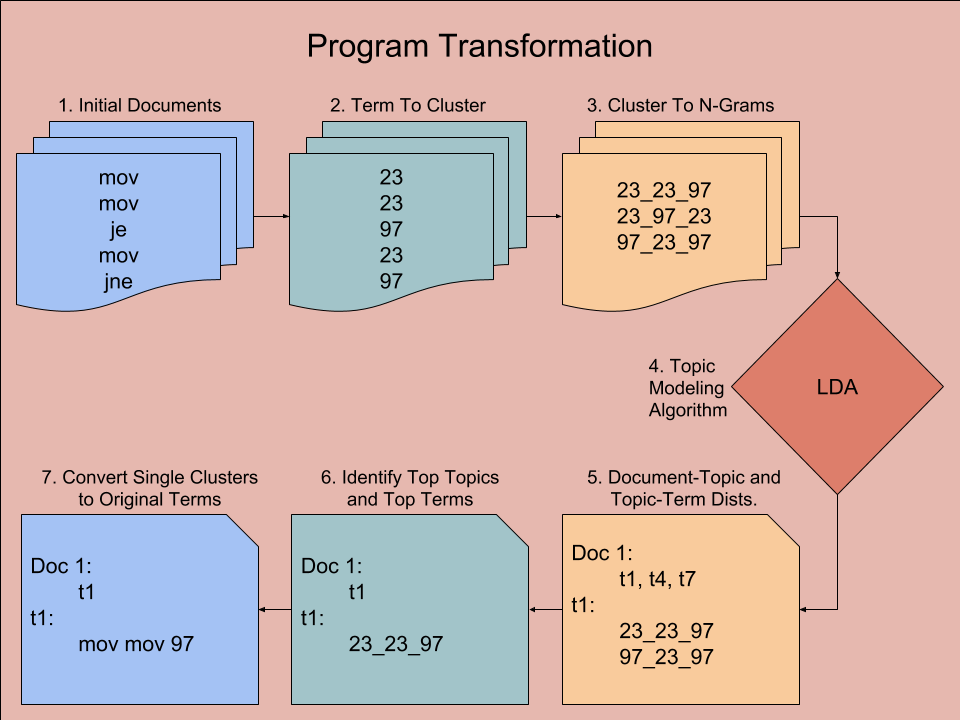
\includegraphics[width=\linewidth]{./figures/transform.png}
  \caption{Flowchart detailing the flow and transformation of information across the entire process. Documents are transformed and analyzed using LDA, and then the transformations are undone to allow for fine-grain interpretability.}
  \label{fig:flow}
\end{figure}

The system described fulfills the requirements of extracting interpretable behavioral components of software in an unsupervised manner. The details of each of the system's components is discussed below.

\subsection{Data and Assembly Instructions}
	\begin{figure}
  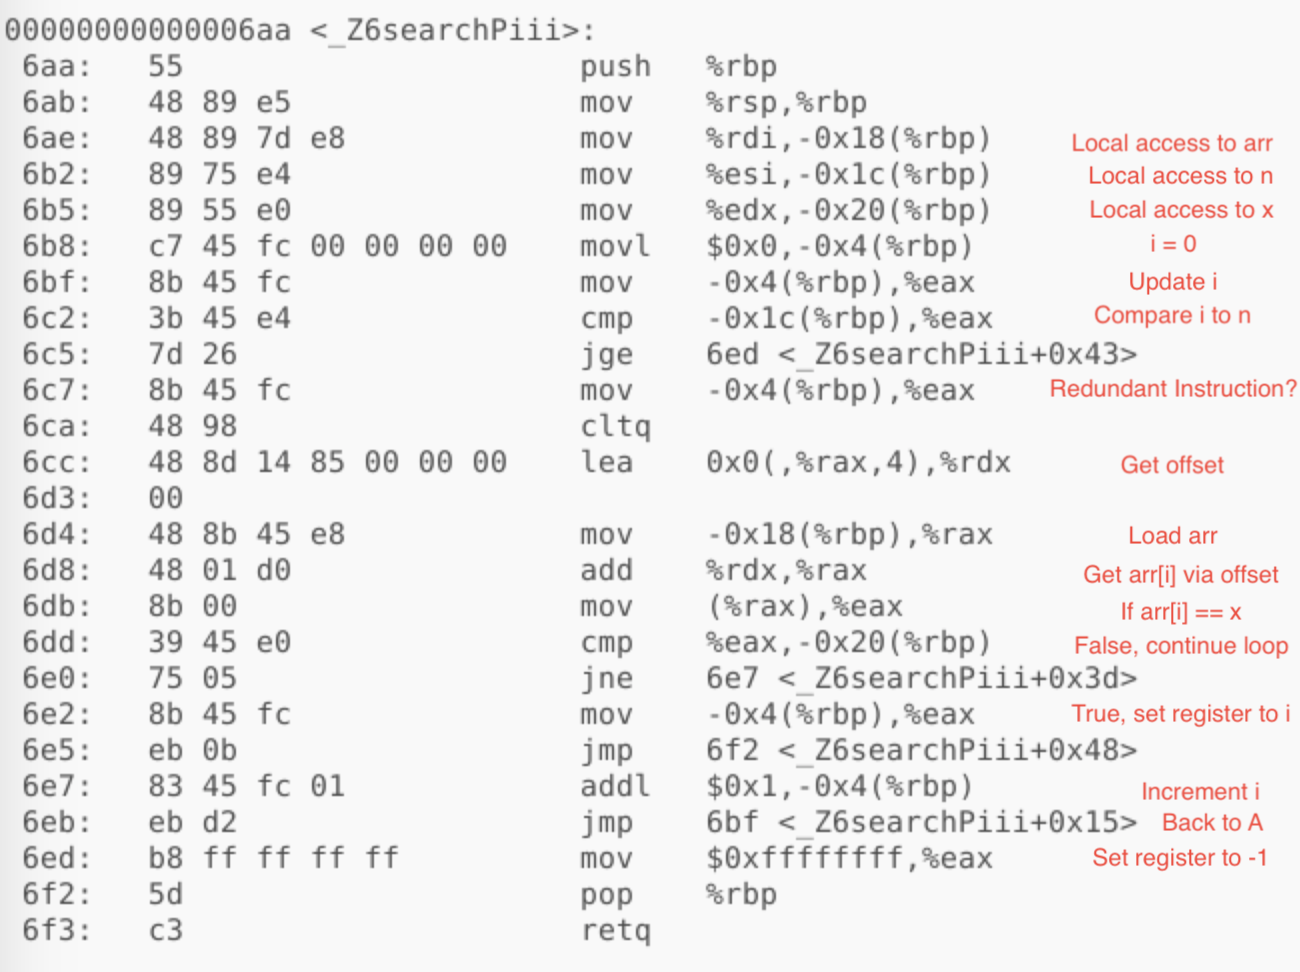
\includegraphics[width=\linewidth]{./figures/Annotated_search_assembly_ATT.png}
  \caption{Annotated version of Linear Search's search function in assembly. Similarities were found in sorting functions with the primary difference being sections of data modification and multiple for-loops.}
  \label{fig:search}
\end{figure}

Before moving towards a specific model, we first wished to see what differences occur between programs with different purposes, such as sorting programs versus searching programs. These two types of programs are two fundamental concepts of many programs and were identified as appropriate vehicles to develop and understand this approach. Initial analyses were performed on a small dataset collected from the Geeks4Geeks Website \cite{geeks}, where C++ samples of major sorting and searching algorithms were downloaded and compiled onto a Ubuntu 64-bit system. A larger dataset was later utilized using ByteWeight's dataset \cite{bao2014byteweight}. 

To understand the differences between programs, we first closely examined one sorting and one searching program to see what differences might exist between their assemblies. Figure \ref{fig:search} shows an annotated version of Linear Search's search function, and when compared with a sorting program such as Selection Sort (which effectively contains a modified version of a linear search as it sorts the program), the primary differences found were multiple for-loops and sections for data modification, something which most, if not all, sorting programs should have, but no realistic searching programs should have, as efficient searching programs should only have one loop, and should not be modifying the data. This formed the basis of our argument: \textit{Programs can be thought of as being made up of a set of underlying components, and these components are in some way shared across all programs.} The order and frequency in which these components occur can enable behavioral comparisons between programs, and understanding the components themselves allows for fine-grain understanding of behavior. The system presented in this work only incorporates the commands themselves so that basic functionality of the software could be understood. Incorporating arguments would allow for a better understanding of command targets (such as specific registers or functions), but would first require abstracting these in a way similar to Symbolic Execution so that program-to-program comparisons can be maintained.

	
\subsection{Word2Vec Embeddings and Clustering}
	Assembly commands also deserve their own form of abstraction, primarily in the context in which they are used. Using sorting as an example, changing a single greater-than comparator to a less-than comparator does not change the fact that the program is sorting, all it changes is the sorting order from increasing to decreasing. In order to allow for greater robustness in program types, our system must be able to take the context in which a specific command is used into account. One of the most effective methods of this is Word2Vec \cite{mikolov2013distributed}, which is able to identify terms used in similar contexts and can even be extrapolated to higher-level relationships (such as man->woman being similar to king->queen). Using the embeddings learned from Word2Vec, we gain a numerical representation of each command's context, with more similar commands sharing similar contexts. 

The small-scale experiment results of Word2Vec are shown in the T-SNE plot in Figure \ref{fig:tsne}. The findings shown in the plot correspond relatively well to human understanding, as most of the jump comparators are close to each other (jle, jg, jge); however, je is actually quite far from the rest of the comparators. We believe this is the result of the small data sample (16 documents) skewing the results. Once the high-dimensional embedding representations of terms were found, we applied hierarchical clustering to them and used our best understanding of command similarity to define the cutting point. Though this approach was adequate to confirm the validity of our system, a more formal study of assembly language usage would be preferred to validate the contexts in which commands are used and how they relate to one another. The results of this are shown in Figure \ref{fig:clust}. Both of these processes are repeated for the larger (about 850 documents) dataset, though the results of those embeddings and clusters are not shown in this paper as the images are too cluttered to be meaningfully presented.

\begin{figure}
  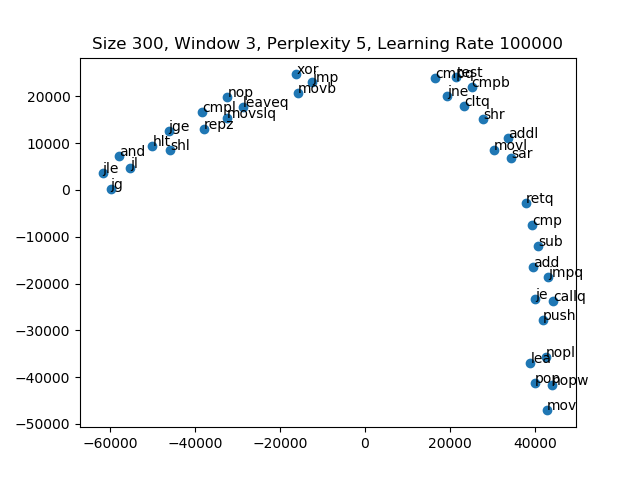
\includegraphics[width=\linewidth]{./figures/tsne_small.png}
  \caption{T-SNE plot of small-scale data Word2Vec results.}
  \label{fig:tsne}
\end{figure}

\begin{figure}
  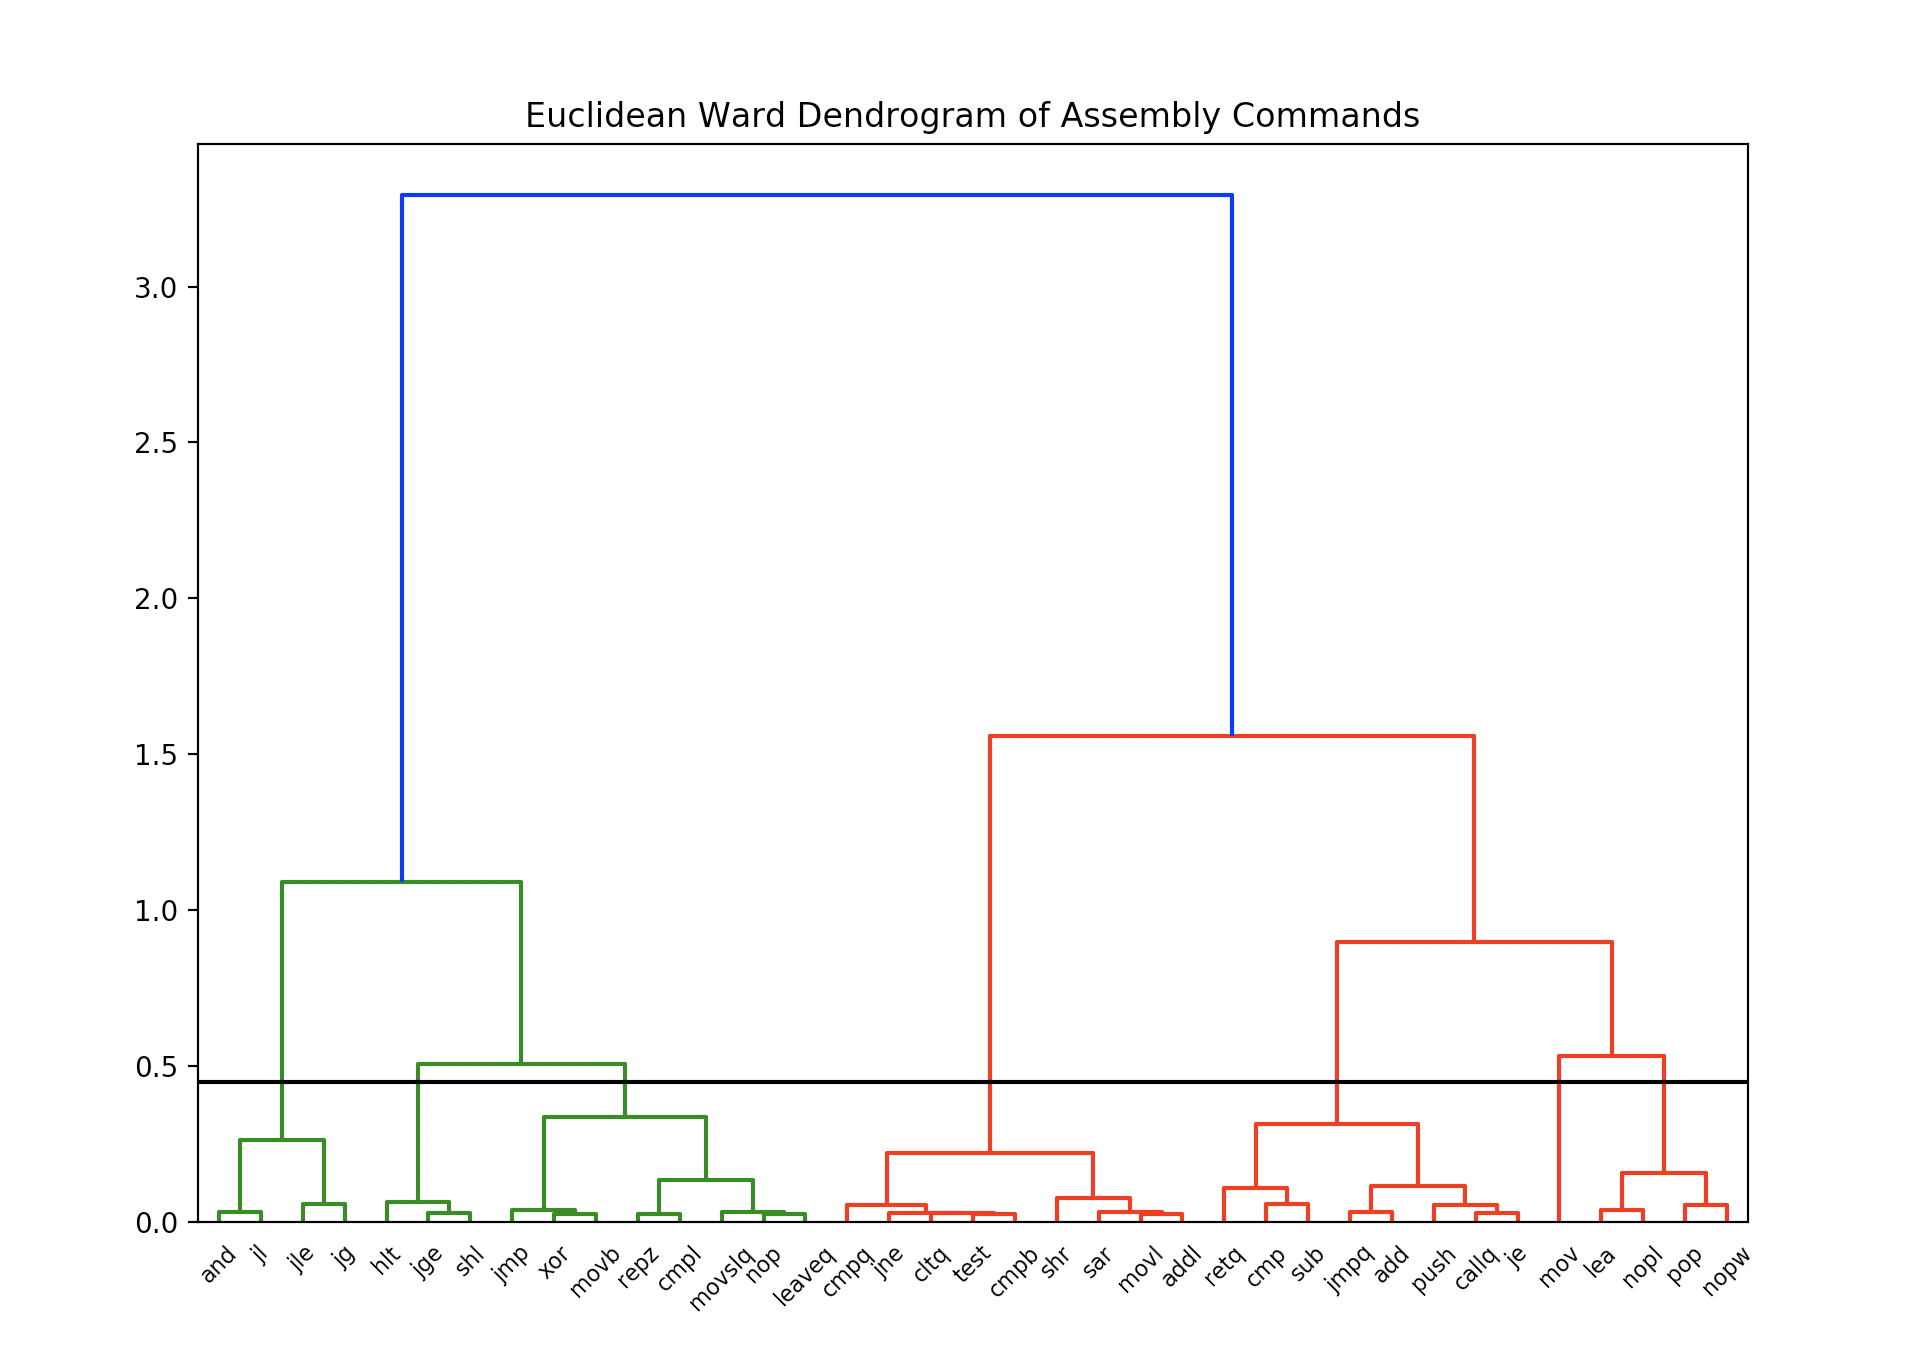
\includegraphics[width=\linewidth]{./figures/clust_small.png}
  \caption{Hierarchical Clustering results of the small dataset.}
  \label{fig:clust}
\end{figure}
	
\subsection{N-Grams}
	After converting the assembly commands to their corresponding cluster ID's, a way to have components with interpretable behavior was desired. Individual commands carry little meaning beyond their intended purpose, as one cannot extrapolate the meaning of a single "mov" or "pop" statement beyond its intended purpose; however, one can derive greater understanding of behavior through sequences of terms rather than singular terms. This brings us to N-Grams, which are sequences of terms (in this case cluster IDs) adjacent to each other (e.g. the 2-grams of "mov addl mov pop" are "mov addl", "addl mov", and "mov pop"). Smaller N-grams are less interpretable than large N-grams, and so a sizeable N must be chosen to maintain interpretability, which for our purposes means N = 8. Unfortunately, this has the side effect of drastically increasing vocabulary, so some caution must be taken.
	
\subsection{LDA and hLDA}
	As we defined programs as being made up sets of behavioral components, and those behaviors are largely unknown to us, we needed a system which would allow us to extract those behaviors in an unsupervised manner. This is actually a well-studied area in languages with NLP approaches in the area called Topic Modeling. Blei \textit{et al.} \cite{blei2003latent} developed a method for unsupervised topic modeling called Latent Dirichlet Allocation and would later expand upon it by developing Hierarchical Latent Dirichlet Allocation (hLDA) \cite{griffiths2004hierarchical}. LDA essentially considers each document to be made up of some weighting of latent topics and each topic to be made up of some weighting of terms. Then, it finds the distribution on these weightings which can be used for inference. hLDA is a hierarchical variant which adds the idea that topics are actually structured in a hierarchy. This approach is more akin to software than flat topics; however, there are not many performant hLDA libraries available for larger datasets. This led to a focus on LDA for the time being. LDA has more performant versions available, such as Microsoft's LightLDA \cite{yuan2015lightlda}, which we utilize in our analyses on the larger dataset.
	
